\documentclass[a4paper,11pt]{book}
%\documentclass[a4paper,twoside,11pt,titlepage]{book}
\usepackage{listings}
\usepackage[utf8]{inputenc}
\usepackage[spanish]{babel}

% \usepackage[style=list, number=none]{glossary} %
%\usepackage{titlesec}
%\usepackage{pailatino}

\usepackage[
backend=biber,
style=alphabetic,
sorting=ynt
]{biblatex}
\addbibresource{bibliografia.bib}

\usepackage{breakcites}
\usepackage{float}

\decimalpoint
\usepackage{dcolumn}
\newcolumntype{.}{D{.}{\esperiod}{-1}}
\makeatletter
\addto\shorthandsspanish{\let\esperiod\es@period@code}
\makeatother


%\usepackage[chapter]{algorithm}
\RequirePackage{verbatim}
%\RequirePackage[Glenn]{fncychap}
\usepackage{fancyhdr}
\usepackage{graphicx}
\graphicspath{./doc/imagenes}
\usepackage{afterpage}

\usepackage{longtable}

\usepackage[pdfborder={000}]{hyperref} %referencia

% ********************************************************************
% Re-usable information
% ********************************************************************
\newcommand{\myTitle}{Aplicación de renderizado 3D\xspace}
\newcommand{\myDegree}{Grado en ingeniería informática\xspace}
\newcommand{\myName}{Pablo Cantudo Gómez\xspace}
\newcommand{\myProf}{Juan Carlos Torres Cantero y Luis López Escudero\xspace}
%\newcommand{\mySupervisor}{Put name here\xspace}
\newcommand{\myFaculty}{Escuela Técnica Superior de Ingenierías Informática y de
Telecomunicación\xspace}
\newcommand{\myFacultyShort}{E.T.S. de Ingenierías Informática y de
Telecomunicación\xspace}
\newcommand{\myDepartment}{Departamento de Lenguajes y Sistemas Informáticos\xspace}
\newcommand{\myUni}{\protect{Universidad de Granada}\xspace}
\newcommand{\myLocation}{Granada\xspace}
\newcommand{\myTime}{\today\xspace}
\newcommand{\myVersion}{Version 0.1\xspace}


\usepackage{dirtree}
\usepackage{url}
\usepackage{colortbl,longtable}
\usepackage[stable]{footmisc}
\usepackage{index}

\makeindex
\usepackage[toc,nonumberlist]{glossaries}
\makeglossaries

% Definición de comandos que me son tiles:
%\renewcommand{\indexname}{Índice alfabético}
%\renewcommand{\glossaryname}{Glosario}

\pagestyle{fancy}
\fancyhf{}
\fancyhead[LO]{\leftmark}
\fancyhead[RE]{\rightmark}
\fancyhead[RO,LE]{\textbf{\thepage}}
\renewcommand{\chaptermark}[1]{\markboth{\textbf{#1}}{}}
\renewcommand{\sectionmark}[1]{\markright{\textbf{\thesection. #1}}}

\setlength{\headheight}{1.5\headheight}

\newcommand{\HRule}{\rule{\linewidth}{0.5mm}}
%Definimos los tipos teorema, ejemplo y definición podremos usar estos tipos
%simplemente poniendo \begin{teorema} \end{teorema} ...
\newtheorem{teorema}{Teorema}[chapter]
\newtheorem{ejemplo}{Ejemplo}[chapter]
\newtheorem{definicion}{Definición}[chapter]

\definecolor{gray97}{gray}{.97}
\definecolor{gray75}{gray}{.75}
\definecolor{gray45}{gray}{.45}
\definecolor{gray30}{gray}{.94}

\lstset{ frame=Ltb,
     framerule=0.5pt,
     aboveskip=0.5cm,
     framextopmargin=3pt,
     framexbottommargin=3pt,
     framexleftmargin=0.1cm,
     framesep=0pt,
     rulesep=.4pt,
     backgroundcolor=\color{gray97},
     rulesepcolor=\color{black},
     %
     stringstyle=\ttfamily,
     showstringspaces = false,
     basicstyle=\scriptsize\ttfamily,
     commentstyle=\color{gray45},
     keywordstyle=\bfseries,
     %
     numbers=left,
     numbersep=6pt,
     numberstyle=\tiny,
     numberfirstline = false,
     breaklines=true,
   }
 
% minimizar fragmentado de listados
\lstnewenvironment{listing}[1][]
   {\lstset{#1}\pagebreak[0]}{\pagebreak[0]}

\lstdefinestyle{CodigoC}
   {
	basicstyle=\scriptsize,
	frame=single,
	language=C,
	numbers=left
   }
\lstdefinestyle{python}
   {
	basicstyle=\small,
	frame=single,
	backgroundcolor=\color{gray30},
	language=C++,
	numbers=left
   }

 
\lstdefinestyle{Consola}
   {basicstyle=\scriptsize\bf\ttfamily,
    backgroundcolor=\color{gray30},
    frame=single,
    numbers=none
   }


\newcommand{\bigrule}{\titlerule[0.5mm]}


%Para conseguir que en las páginas en blanco no ponga cabecerass
\makeatletter
\def\clearpage{%
  \ifvmode
    \ifnum \@dbltopnum =\m@ne
      \ifdim \pagetotal <\topskip
        \hbox{}
      \fi
    \fi
  \fi
  \newpage
  \thispagestyle{empty}
  \write\m@ne{}
  \vbox{}
  \penalty -\@Mi
}
\makeatother

\usepackage{pdfpages}
\begin{document}
\begin{titlepage}
 
 
\newlength{\centeroffset}
\setlength{\centeroffset}{-0.5\oddsidemargin}
\addtolength{\centeroffset}{0.5\evensidemargin}
\thispagestyle{empty}

\noindent\hspace*{\centeroffset}\begin{minipage}{\textwidth}

\centering

\includegraphics[width=0.9\textwidth]{imagenes/logo.png}\\[1.4cm]

\textsc{ \Large TRABAJO FIN DE GRADO\\[0.2cm]}
\textsc{ GRADO EN INGENIERÍA INFORMÁTICA}\\[1cm]
% Upper part of the page
% 
% Title
{\Huge\bfseries \\ Desarrollo de una aplicaci´on
de modelado 3D}
\noindent\rule[-1ex]{\textwidth}{3pt}\\[3.5ex]
{\large\bfseries Motor de renderizado en tiempo real basada en SDFs}
\end{minipage}

\vspace{2.5cm}
\noindent\hspace*{\centeroffset}\begin{minipage}{\textwidth}
\centering

\textbf{Autor}\\ {Pablo Cantudo Gómez}\\[2.5ex]
\textbf{Directores}\\
{Juan Carlos Torres Cantero y Luis López Escudero\\}\\[2cm]

\includegraphics[width=0.3\textwidth]{imagenes/etsiit_logo.png}\\[0.1cm]
\textsc{Escuela Técnica Superior de Ingenierías Informática y de Telecomunicación}\\
\textsc{---}\\
Granada, Septiembre de 2025
\end{minipage}
%\addtolength{\textwidth}{\centeroffset}
%\vspace{\stretch{2}}
\end{titlepage}



\thispagestyle{empty}

\begin{center}
{\large\bfseries Desarrollo software de una aplicación de modelado 3d basada en Signed Distance Funtion (sdf) \\ Motor de renderizado en tiempo real usando Dawn, C++ y WebGPU }\\
\end{center}
\begin{center}
Pablo Cantudo Gómez\\
\end{center}

\vspace{0.7cm}

\vspace{0.5cm}
\noindent\textbf{Palabras clave}: \textit{SDF}, \textit{WebGPU}, \textit{C++}, \textit{ray marching}, \textit{motor de renderizado}
\vspace{0.7cm}

\noindent\textbf{Resumen}\\
\break
Este trabajo presenta el desarrollo de \textit{Copper}, un motor de renderizado 3D en tiempo real implementado en C++ utilizando la API WebGPU a trav\'es de Dawn.
El motor emplea t\'ecnicas de \textit{ray marching} sobre funciones de distancia con signo (SDF), lo que permite una representaci\'on eficiente y flexible de geometr\'ia 
 tridimensional. Una de las principales ventajas de utilizar SDF es la capacidad de expresar de forma directa y compacta operaciones booleanas entre primitivas geom\'etricas
  ---como uniones, intersecciones o diferencias--- mediante simples expresiones algebraicas. Adem\'as, a diferencia de los m\'etodos tradicionales basados en mallas o 
  pol\'igonos, las SDF permiten aplicar operaciones booleanas suaves, como la uni\'on con suavizado (\textit{smooth union}), 
  de forma pr\'acticamente trivial desde el punto de vista computacional.
\bigbreak
Este enfoque simplifica notablemente la construcci\'on de formas complejas, evitando problemas t\'ipicos de la computaci\'on geom\'etrica como el manejo 
de v\'ertices, normales o topolog\'ias complejas. Tambi\'en se facilita la animaci\'on y transformaci\'on de objetos mediante funciones continuas. El motor 
incluye un sistema de sombreado en WGSL, con soporte para sombras suaves, operaciones modulares sobre la escena, seleccion de objetos, carga y guardado de modelos. Los resultados demuestran que
el uso de SDF no solo ofrece un modelo m\'as elegante para definir geometr\'ia, sino que permite construir escenas visualmente complejas con menos c\'odigo y una mayor expresividad gr\'afica.
En conjunto, el sistema demuestra la viabilidad t\'ecnica y creativa del uso de SDF en entornos modernos.
\cleardoublepage

\begin{center}
	{\large\bfseries Development of a 3D modeling application based on Signed Distance Functions (SDF) \\ Real-time rendering engine using Dawn, C++ and WebGPU}\\
\end{center}
\begin{center}
	Pablo Cantudo Gómez\\
\end{center}
\vspace{0.5cm}
\noindent\textbf{Keywords}: \textit{SDF}, \textit{WebGPU}, \textit{C++}, \textit{ray marching}, \textit{rendering engine}
\vspace{0.7cm}

\noindent\textbf{Abstract}\\
\break
This work presents the development of Copper, a real-time 3D rendering engine implemented in C++ using the WebGPU API through Dawn.
The engine employs ray marching techniques over Signed Distance Functions/Fields (SDF), enabling an efficient and flexible representation of three-dimensional geometry.
One of the main advantages of using SDF is the ability to directly and compactly express Boolean operations between geometric primitives ---such as unions, intersections, or differences--- through simple algebraic expressions.
Furthermore, unlike traditional mesh- or polygon-based methods, SDF allows for smooth Boolean operations, such as smooth union, in a virtually trivial manner from a computational standpoint.
\bigbreak
This approach greatly simplifies the construction of complex shapes, avoiding typical problems in geometric computing such as handling vertices, normals, or complex topologies.
It also facilitates the animation and transformation of objects through continuous functions.
The engine includes a shading system in WGSL, with support for soft shadows, modular scene operations, object selection, and model loading and saving.
The results show that the use of SDF not only offers a more elegant model for defining geometry, but also enables the creation of visually complex scenes with less code and greater graphical expressiveness.
Overall, the system demonstrates the technical and creative feasibility of using SDF in modern environments.

\cleardoublepage

\thispagestyle{empty}

\noindent\rule[-1ex]{\textwidth}{2pt}\\[4.5ex]

D. \textbf{Tutora/e(s)}, Profesor(a) del ...

\vspace{0.5cm}

\textbf{Informo:}

\vspace{0.5cm}

Que el presente trabajo, titulado \textit{\textbf{Chief}},
ha sido realizado bajo mi supervisión por \textbf{Estudiante}, y autorizo la defensa de dicho trabajo ante el tribunal
que corresponda.

\vspace{0.5cm}

Y para que conste, expiden y firman el presente informe en Granada a Junio de 2018.

\vspace{1cm}

\textbf{El/la director(a)/es: }

\vspace{5cm}

\noindent \textbf{(nombre completo tutor/a/es)}

\chapter*{Agradecimientos}
Quiero expresar mi agradecimiento a todas las personas que han contribuido directa o indirectamente a la realización de este trabajo.\break

En primer lugar, a mi tutor Juan Carlos Torres Cantero y cotutor Luis López Escudero por la ayuda durante el desarrollo y la correci\'on del proyecto,
a mis amigos por las discusiones y las ideas, y a mi familia por su apoyo incondicional.\break

 Finalmente, me gustaría mencionar a la comunidad de desarrolladores y recursos abiertos, especialmente los foros, artículos y proyectos relacionados con WebGPU, SDF y ray marching,
 cuya documentación y ejemplos han sido una fuente de aprendizaje invaluable.




%\frontmatter
\tableofcontents
\listoffigures
%\listoftables
%
%\mainmatter
%\setlength{\parskip}{5pt}

\chapter{Introducción}
El desarrollo de los gráficos tridimensionales por computadora ha sido un campo de investigación activo y en constante evolución desde sus inicios.\\
La capacidad de crear representaciones visuales de objetos y escenas en tres dimensiones ha revolucionado diversas industrias, desde el entretenimiento hasta la medicina y la ingeniería.\\
A medida que la tecnología avanza, también lo hacen las técnicas y herramientas utilizadas para generar gráficos 3D, lo que plantea nuevos desafíos y oportunidades para los investigadores y desarrolladores.

En sus inicios, la generación de gráficos 3D estaba limitada por la capacidad de cómputo y se basaba en \textit{pipelines} gráficos fijos compuestos por etapas de transformación, iluminación y rasterización.\\
Posteriormente, con la llegada de los \textit{shaders} programables en GPU (Nvidia GeForce 3 en 2001), fue posible sustituir los \textit{pipelines} fijos por \textit{pipelines} programables, lo que abrió un abanico de posibilidades para la creación de efectos visuales complejos y personalizados, como los algoritmos no basados en polígonos.\\
Esto impulsó la investigación en técnicas de representación más avanzadas, como el \textit{ray tracing} y, en particular, el \textit{ray marching}.

En el contexto del renderizado basado en funciones implícitas, las \textit{Signed Distance Functions} (SDF) no son una invención reciente, sino que tienen sus raíces en trabajos mucho más antiguos.\\
El concepto de combinar funciones implícitas mediante operaciones booleanas se remonta al trabajo de Ricci en 1972~\cite{Ricci:1973:CGC}, y fue ampliado en 1989 por B.~Wyvill y G.~Wyvill con el modelado de \textit{soft objects}~\cite{wyvill1989}.\\
Ese mismo año, Sandin, Hart y Kauffman aplicaron \textit{ray marching} a SDF para renderizar fractales tridimensionales~\cite{hart1989ray}.\\
Posteriormente, en 1995, Hart documentó de nuevo la técnica, a la que denominó \textit{Sphere Tracing}~\cite{hart1996}.

La popularización moderna de las SDF en el ámbito del \textit{renderizado en tiempo real} se debe en gran parte a la comunidad \textit{demoscene}, especialmente a partir de mediados de la década de 2000.\\
Trabajos como el de Crane (2005) y Evans (2006) introdujeron la idea de restringir el campo a una distancia euclidiana real, mejorando el rendimiento y la calidad visual.\\
Sin embargo, el uso de esta técnica no está tan extendido en aplicaciones de renderizado en tiempo real, a pesar de su potencial para crear gráficos visuales y eficientes.
\section{Motivación}

Como cualquier persona nacida en los dos mil, he crecido rodeado de videojuegos y el avance en la tecnología de gráficos 3D ha sido un aspecto fascinante de esta industria. 
Durante la carrera de informática, estudié diversas asignaturas relacionadas con gráficos por computadora, cuyos proyectos despertaron y consolidaron mi interés en este campo.

El desarrollo de motores gráficos y técnicas de renderizado siempre me ha resultado un área especialmente atractiva, no solo por su complejidad técnica, 
sino también por el impacto directo que tienen en sectores como el entretenimiento, la simulación o la realidad virtual. A lo largo de mis estudios me encontré con herramientas muy potentes, 
pero también con la dificultad que implica dominarlas o adaptarlas a entornos experimentales. Esto me llevó a plantearme la posibilidad de crear una aplicación propia que sirviera 
como espacio de exploración.

La motivación principal de este trabajo es profundizar en tecnologías emergentes, en concreto \textbf{WebGPU}, un estándar reciente que promete unificar el desarrollo gráfico multiplataforma 
con un acceso eficiente a las GPU modernas. Asimismo, me interesaba experimentar con el modelado mediante \textbf{funciones de distancia (SDF)}, que representan una alternativa flexible al 
modelado poligonal clásico. Considero que la combinación de ambas tecnologías constituye un terreno de investigación con un gran potencial, tanto en aplicaciones prácticas como en entornos 
educativos.

Finalmente, este proyecto me ofrece la oportunidad de afianzar mis conocimientos en programación gráfica, shaders y arquitecturas modernas de GPU, a la vez que desarrollo un software propio 
que pueda servir de base para futuros trabajos de investigación o aplicaciones más complejas en el ámbito del diseño 3D.

\section{Descripción del problema}

El campo del modelado y renderizado 3D ha estado tradicionalmente dominado por herramientas complejas y de gran envergadura, como Blender, Maya o 3ds Max. Si bien estas aplicaciones 
ofrecen una gran potencia y versatilidad, presentan también limitaciones importantes: requieren elevados recursos de hardware, poseen curvas de aprendizaje pronunciadas y no siempre resultan 
adecuadas para entornos de experimentación ligera o proyectos educativos.

Por otro lado, las API gráficas más extendidas, como OpenGL o DirectX, han demostrado su eficacia a lo largo de los años, pero presentan restricciones en cuanto a eficiencia y portabilidad 
en plataformas modernas. El reciente estándar \textbf{WebGPU} surge como respuesta a estas carencias, ofreciendo un modelo de programación más cercano al hardware y multiplataforma, con el 
objetivo de unificar el desarrollo gráfico en navegadores y aplicaciones nativas.

En el ámbito del modelado, el paradigma poligonal sigue siendo el más utilizado, pero alternativas como las \textbf{funciones de distancia (SDF)} permiten representar geometrías complejas 
de manera más compacta y flexible, facilitando la combinación de primitivas y operaciones booleanas. Sin embargo, la integración de estas técnicas en aplicaciones prácticas 
todavía es limitada, especialmente en combinación con tecnologías emergentes como WebGPU.

El problema que aborda este trabajo consiste en la falta de herramientas ligeras que sirvan como demostración y entorno de experimentación para el modelado y renderizado basados en SDF 
sobre WebGPU.

\section{Objetivos}

\subsection*{Objetivo general}
El objetivo principal de este Trabajo de Fin de Grado es el desarrollo de una aplicación de diseño 3D basada en \textbf{WebGPU} y en técnicas de 
\textbf{modelado mediante funciones de distancia (SDF)}, que permita explorar y demostrar el potencial de estas tecnologías como alternativa al modelado poligonal clásico y 
como herramienta de experimentación en el ámbito de los gráficos por computadora.

\subsection*{Objetivos específicos}
Para alcanzar este objetivo general, se plantean los siguientes objetivos específicos:

\begin{itemize}
    \item Investigar y comprender en profundidad el funcionamiento de la API WebGPU y su integración en aplicaciones nativas mediante la librería Dawn.
    \item Diseñar e implementar un motor de renderizado basado en \textit{ray marching} sobre funciones de distancia, capaz de representar primitivas y 
    combinaciones mediante operaciones booleanas y suaves.
    \item Incorporar técnicas de sombreado y efectos visuales (iluminación, sombras suaves) que mejoren la calidad del renderizado.
    \item Desarrollar una interfaz gráfica sencilla que permita al usuario interactuar con la escena y manipular las primitivas.
\end{itemize}


\section{Estructura de la memoria}

La presente memoria se organiza en los siguientes capítulos:

\begin{itemize}
    \item \textbf{Introducción:} Se expone el contexto del trabajo, la motivación, los objetivos planteados y la justificación de la elección de las tecnologías empleadas.
    \item \textbf{Fundamentos teóricos:} Se revisan los conceptos clave de modelado y renderizado 3D, las funciones de distancia (\textit{Signed Distance Functions, SDF}) y el estándar WebGPU, contextualizando el trabajo en el estado actual de la tecnología.
    \item \textbf{Arquitectura de la aplicación:} Se describe la estructura general de la aplicación Copper, detallando los principales módulos, componentes y la interacción entre ellos.
    \item \textbf{Implementación:} Este capítulo se divide en varias secciones:
    \begin{itemize}
        \item \textbf{Ventana y motor de renderizado:} Se explica el proceso de inicialización de la ventana, integración con Dawn/WebGPU y el desarrollo del motor de renderizado basado en SDF y ray marching.
        \item \textbf{Controles e interacción:} Se detalla la implementación de los controles de cámara y de manipulación de objetos mediante la interfaz gráfica.
        \item \textbf{Shaders y efectos visuales:} Se describe el desarrollo de los shaders WGSL utilizados, incluyendo técnicas de sombreado, iluminación y efectos visuales implementados.
    \end{itemize}
    \item \textbf{Conclusiones y trabajos futuros:} Se realiza un balance del trabajo realizado, se revisa el grado de cumplimiento de los objetivos y se plantean posibles líneas de investigación y desarrollo futuras.
    \item \textbf{Bibliografía y anexos:} Se recopilan las referencias bibliográficas consultadas y se incluyen materiales complementarios relevantes para la comprensión y reproducibilidad del trabajo.
\end{itemize}
\chapter{Fundamentos teóricos}

El modelado y renderizado en 3D es posible gracias a una serie de técnicas
matemáticas y computacionales que permiten representar, manipular y visualizar
geometría en entornos virtuales. Copper se basa en el modelado mediante
funciones de distancia con signo (SDF), el renderizado por \textit{ray
    marching} y el uso del estándar gráfico WebGPU, usando Dawn para aplicarlo a
C++. Este capítulo describe en profundidad cada uno de estos fundamentos.

\section{Modelado tridimensional: Paradigmas y fundamentos}

El modelado tridimensional tradicional se basa en mallas poligonales, en las
que los objetos se representan mediante listas de vértices, aristas y caras
conectadas para formar la superficie. Herramientas como \textit{Blender},
\textit{Maya}, y \textit{3ds Max} utilizan este enfoque, que ofrece gran
flexibilidad para la edición y animación, pero que implica la gestión explícita
de la topología, el almacenamiento de grandes cantidades de datos y una
complejidad elevada para ciertas operaciones.

Como alternativa, existen los métodos de representación implícita, como los
campos de distancia con signo (\textit{Signed Distance Fields, SDF}). Una SDF
es una función $f(\vec{x})$ que, para cada punto $\vec{x}$ del espacio,
devuelve la distancia mínima a la superficie del objeto. El signo indica si el
punto está en el interior (negativo), sobre la superficie (cero) o en el
exterior (positivo). Este enfoque permite describir objetos mediante
expresiones matemáticas, simplificando la combinación y manipulación de
geometría compleja.

\section{Funciones de distancia con signo (SDF)}

Las SDF asignan a cada punto del espacio la distancia mínima a una superficie
implícita. Formalmente, para una función $f(\vec{x})$, la superficie se define
como el conjunto de puntos donde $f(\vec{x}) = 0$. Las SDF permiten describir
primitivas básicas como:

\begin{itemize}
    \item \textbf{Esfera}: $f_{esfera}(\vec{x}) = ||\vec{x} - \vec{c}|| - r$, donde $\vec{c}$ es el centro y $r$ el radio.
    \item \textbf{Caja}: $f_{caja}(\vec{x}) = ||\max(|\vec{x} - \vec{c}| - \vec{s}, 0)|| + \min(\max(d_x, \max(d_y, d_z)), 0)$, donde $\vec{s}$ es el tamaño.
    \item \textbf{Cilindro, cono, plano...}: Cada primitiva se expresa como una función matemática que determina la distancia a su superficie.
\end{itemize}

Y también pueden combinarse empleando operadores booleanos y suaves:

\begin{itemize}
    \item \textbf{Unión}: $f_{union}(a, b) = \min(a, b)$
    \item \textbf{Intersección}: $f_{inter}(a, b) = \max(a, b)$
    \item \textbf{Resta}: $f_{resta}(a, b) = \max(a, -b)$
    \item \textbf{Unión suave}: Interpolación entre distancias y colores para crear transiciones continuas.
\end{itemize}

Las SDF son especialmente potentes para casos de generación procedural,
efectos visuales, física, simulaciones y renderizado implícito, permitiendo la
composición jerárquica de formas y la aplicación de transformaciones a nivel
funcional.

\section{Ray Marching}

El \textit{ray marching} es una técnica de renderizado que avanza iterativamente un rayo en el espacio hasta aproximar la intersección con
una superficie implícita. El procedimiento puede describirse en los siguientes
pasos:

\begin{enumerate}
    \item Lanzar un rayo desde la cámara en una dirección determinada.
    \item Evaluar la distancia para el siguiente punto a lo largo del rayo.
    \item Avanzar el punto a lo largo del rayo una distancia igual al valor obtenido.
    \item Repetir hasta que la distancia sea menor que un umbral (colisión con la
          superficie) o se alcance un límite de pasos o distancia máxima.
\end{enumerate}

Este método sumado a las SDF se llama sphere tracing, en este caso la distancia devuelta por la SDF se utiliza para avanzar el rayo de manera óptima.

\subsection{Ray Tracing}

A diferencia del ray marching, el ray tracing cálcula la primera intersección exacta entre el rayo y las primitivas geométricas de la escena. 
Este método es especialmente eficiente para escenas donde la geometría está definida de forma explícita, como mallas poligonales.
El procedimiento es similar al ray marching, se lanza un rayo desde la cámara, pero esta vez en vez de avanzar iterativamente,
se calcula cual es el primer objeto con el que colisionaría el rayo.

El ray tracing no se puede usar con SDF, ya que esta solo devuelve la distancia al objeto más cercano.

\subsection{Sphere Tracing}

La técnica de \textbf{sphere tracing}, introducida por Hart, es una variante
eficiente de ray marching. Utiliza la propia SDF para calcular el avance óptimo
en cada paso del rayo. En cada iteración, la distancia devuelta por la SDF se
interpreta como el radio de una esfera libre de obstáculos centrada en el punto
actual. Así, el rayo puede avanzar exactamente esa distancia sin riesgo de
atravesar ninguna superficie.

Sphere tracing es especialmente útil en escenas donde las funciones de
distancia son suaves y bien definidas, permitiendo renderizar geometría
compleja con costes computacionales bajos. Sin embargo, en superficies muy
delgadas o SDFs poco continuas, el algoritmo puede avanzar muy poco en cada
paso, reduciendo la eficiencia y generando artefactos visuales.

\begin{figure}[H]
    \centering
    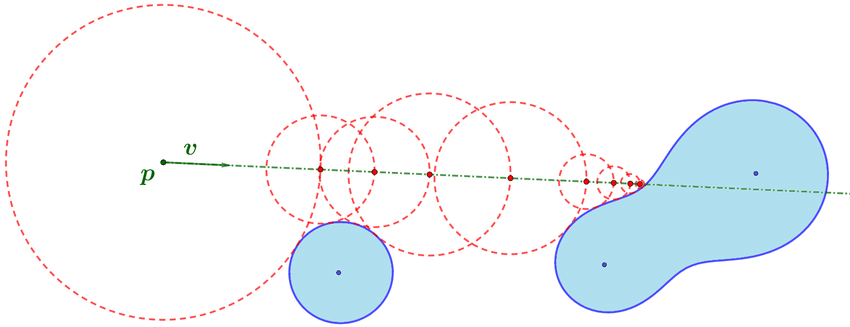
\includegraphics[width=0.6\textwidth]{sphere_tracing.png}
    \caption{Representación visual del algoritmo de sphere tracing, en el que cada círculo representa el rango libre de obstáculos determinado por la SDF.}
    \label{fig:sphere-tracing}
\end{figure}

\subsection{Ventajas y limitaciones de las SDF}

Las SDF ofrecen varias ventajas sobre los métodos de modelado tradicionales:

\begin{itemize}
    \item \textbf{Compacidad}: Las SDF se definen por fórmulas matemáticas en lugar de listas de vértices, lo que reduce el espacio necesario para describir objetos complejos.
    \item \textbf{Facilidad de combinación}: La geometría puede combinarse empleando operadores matemáticos (unión, intersección, resta) de forma eficiente y expresiva.
    \item \textbf{Transformaciones geométricas}: Las transformaciones como traslación, rotación y escalado se aplican directamente sobre la función, facilitando la manipulación.
    \item \textbf{Cálculo de normales}: La normal en la superficie se obtiene como el gradiente de la función de distancia, lo que simplifica el cálculo de iluminación.
    \item \textbf{Flexibilidad}: Permiten crear transiciones suaves entre objetos mediante operadores suavizados, lo que es difícil de lograr con mallas.
\end{itemize}

Pero también presentan diferentes limitaciones a la hora de representar geometría:

\begin{itemize}
    \item \textbf{Precision y aliasing}: El umbral de colisión y el número de pasos afectan la calidad de la imagen y pueden causar aliasing o superficies rugosas.
    \item \textbf{Superficies delgadas}: Si la SDF varía abruptamente o la superficie es muy fina, el avance óptimo se reduce y el número de pasos aumenta significativamente.
    \item \textbf{Efectos avanzados}: Efectos como la refracción y la reflexión requieren múltiples rayos y aumentan el coste computacional.
    \item \textbf{Desempeño}: El rendimiento depende de la complejidad de las funciones SDF y del número de objetos en escena.
\end{itemize}

\section{WebGPU: Acceso moderno a la GPU}

WebGPU es un estándar gráfico de nueva generación que proporciona acceso
eficiente y multiplataforma a la GPU, tanto en navegadores como en aplicaciones
nativas. Surge como respuesta a las limitaciones de APIs tradicionales
como OpenGL y DirectX, ofreciendo mayor control sobre el hardware, mejor
rendimiento y portabilidad.

\subsection{Motivación y principios de diseño}

WebGPU fue diseñado para proporcionar los siguientes atributos a los desarrolladores:

\begin{itemize}
    \item \textbf{Multiplataforma}: Disponible en Windows, Linux, macOS y en navegadores modernos (Chrome, Firefox, Safari).
    \item \textbf{Eficiencia}: Permite describir el flujo de datos entre la CPU y la GPU mediante buffers y pipelines, minimizando el coste de las llamadas de función y la sobrecarga del sistema.
    \item \textbf{Seguridad y portabilidad}: WebGPU abstrae detalles específicos del hardware, garantizando que el mismo código funcione en diferentes dispositivos y plataformas.
    \item \textbf{Modelo explícito}: El usuario configura directamente los recursos (buffers, texturas, pipelines) y controla el ciclo de vida de los datos, permitiendo optimizaciones avanzadas.
\end{itemize}

En contraste con OpenGL/WebGL, WebGPU obliga a definir explícitamente los
recursos y su uso, lo que mejora la seguridad y el rendimiento pero requiere
una mayor comprensión del modelo de GPU.

\subsection{Conceptos clave de WebGPU}

\begin{itemize}
    \item \textbf{Buffers}: Áreas de memoria para almacenar datos como vértices, índices y uniforms.
    \item \textbf{Textures}: Imágenes y mapas de datos que pueden ser leídos y escritos por la GPU.
    \item \textbf{Bind Groups}: Conjuntos de recursos que se vinculan a los shaders, permitiendo el acceso eficiente a datos en la GPU.
    \item \textbf{Pipelines}: Describen la secuencia de operaciones gráficas, incluyendo shaders, estados de rasterización y configuración de recursos.
    \item \textbf{Shaders}: Programas ejecutados en la GPU que transforman datos y calculan colores de píxeles.
    \item \textbf{Command Buffers}: Secuencias de instrucciones que la GPU ejecuta para renderizar o procesar datos.
\end{itemize}

WebGPU utiliza el lenguaje WGSL (\textit{WebGPU Shading Language}) para la
programación de shaders, ofreciendo una sintaxis moderna y expresiva adaptada a
las necesidades de la computación gráfica actual.

\section{Shaders y lenguaje WGSL}

Los \textbf{shaders} son programas que ejecutan operaciones matemáticas en la
GPU para transformar vértices, calcular colores y simular efectos visuales. En
WebGPU, los shaders se escriben en WGSL (\textit{WebGPU Shading Language}), un
lenguaje moderno diseñado para expresar funciones de distancia, operadores
booleanos, cálculos de iluminación y efectos visuales de forma eficiente.

\begin{itemize}
    \item \textbf{Vertex shaders}: Transforman posiciones y atributos de vértices.
    \item \textbf{Fragment shaders}: Calculan el color final de cada píxel, aplicando modelos de iluminación como Blinn-Phong, efectos de sombras y combinaciones de SDF.
\end{itemize}

WGSL permite aprovechar la arquitectura de la GPU para realizar renderizado en
tiempo real, combinando eficiencia y expresividad.

\subsection{Dawn: Implementación nativa de WebGPU}

\textbf{Dawn} es una implementación nativa de la API WebGPU desarrollada por Google y la comunidad Chromium\cite{dawn}. Dawn permite ejecutar aplicaciones que usan WebGPU fuera del navegador, proporcionando acceso directo y multiplataforma a la GPU. Es el backend utilizado por Copper para interactuar con WebGPU desde C++.

En Copper, Dawn se integra como una dependencia externa, permitiendo:

\begin{itemize}
    \item \textbf{Creación de instancias de WebGPU}: A través de las clases y funciones de Dawn, Copper inicializa \texttt{wgpu::Instance}, \texttt{wgpu::Device}, y otros objetos fundamentales.
    \item \textbf{Gestión de recursos}: Dawn facilita la creación y gestión de buffers, texturas y pipelines, siguiendo la especificación de WebGPU.
    \item \textbf{Integración con GLFW}: Mediante el módulo \texttt{webgpu-glfw}, Copper conecta la gestión de ventanas de GLFW con las superficies de renderizado de Dawn/WebGPU.
\end{itemize}

El ciclo de inicialización y renderizado en Copper se basa en la creación de la
instancia de Dawn (\texttt{CreateInstance}), la selección de adaptador y
dispositivo (\texttt{GetAdapter}, \texttt{GetDevice}), y la configuración de la
superficie de dibujo (\texttt{ConfigureSurface}). Los comandos de renderizado
se envían a la GPU mediante \texttt{CommandEncoder} y
\texttt{RenderPassEncoder}, siguiendo el modelo de WebGPU.

\section{Herramientas auxiliares}

El desarrollo de aplicaciones gráficas requiere gestionar ventanas, entrada de
usuario y la interfaz gráfica. Copper utiliza las siguientes herramientas:

\begin{itemize}
    \item \textbf{GLFW}: Biblioteca multiplataforma para la gestión de ventanas y eventos, usada a partir de su módulo de Dawn\cite{glfw-docs}.
    \item \textbf{ImGui}: Sistema de interfaz gráfica inmediata para la manipulación interactiva de primitivas y parámetros de escena\cite{imgui}.
    \item \textbf{GLM}: Biblioteca matemática para operaciones con vectores y matrices\cite{glm}.
    \item \textbf{CMake}: Herramienta de compilación y gestión de dependencias\cite{cmake-docs}.
\end{itemize}

Estas herramientas proporcionan la infraestructura básica para la interacción y
visualización dentro del entorno de Copper.
\chapter{Arquitectura del sistema}

La arquitectura de \textbf{Copper} ha sido concebida siguiendo principios de
modularidad, mantenibilidad y claridad estructural. A continuación se detallan
los diferentes módulos que componen el sistema, describiendo su funcionalidad y
las interacciones que mantienen entre sí, con referencias directas al código
fuente.

\section{Módulo Core}

El módulo \textbf{Core} (\texttt{src/core/Core.cpp}, \texttt{src/core/Core.h})
es el responsable de orquestar el ciclo de vida de la aplicación. Sus funciones
principales incluyen:
\begin{itemize}
    \item \textbf{Inicialización}: Llama a los métodos de inicialización de los módulos \texttt{Window} y \texttt{Renderer} para preparar el entorno gráfico y la ventana principal.
    \item \textbf{Bucle principal}: Ejecuta el método \texttt{MainLoop()}, que gestiona los eventos y delega el renderizado de la escena.
    \item \textbf{Gestión de estado}: Permite saber si la aplicación sigue ejecutándose (\texttt{IsRunning()}) y controla el cierre ordenado de recursos (\texttt{Terminate()}).
\end{itemize}

\section{Módulo Window}

El módulo \textbf{Window} (\texttt{src/ui/Window.cpp},
\texttt{src/ui/Window.h}) se encarga de la creación y gestión de la ventana
principal de la aplicación, utilizando GLFW. Sus funciones incluyen:
\begin{itemize}
    \item \textbf{Configuración de la ventana}: Establece parámetros como el tamaño, aspecto y modo de interacción.
    \item \textbf{Gestión de eventos}: Implementa callbacks para eventos de redimensionado y de ratón, que se propagan al módulo \texttt{Renderer}.
    \item \textbf{Interfaz con el sistema}: Abstrae la interacción con el sistema operativo y facilita la obtención de dimensiones y el manejo del ciclo de vida de la ventana.
\end{itemize}
Esto permite que la ventana sea independiente del motor de renderizado y fácil de modificar o ampliar.

\section{Módulo Renderer}

El \textbf{Renderer} (\texttt{src/core/Renderer.cpp},
\texttt{src/core/Renderer.h}) es el motor gráfico del sistema. Sus principales
responsabilidades son:
\begin{itemize}
    \item \textbf{Inicialización de gráficos}: Configura el contexto de WebGPU, las superficies y los buffers necesarios para el renderizado.
    \item \textbf{Ciclo de renderizado}: Gestiona el bucle de renderizado, actualizando los datos de la escena y llamando a la función \texttt{Render()} en cada frame.
    \item \textbf{Gestión de uniforms}: Actualiza los uniforms (matriz MVP, posición de luz, tamaño de ventana, etc.) y los envía al shader.
    \item \textbf{Coordinación de módulos}: Instancia y gestiona los módulos \texttt{Camera}, \texttt{CameraController}, \texttt{GizmoControls}, \texttt{Coder} e \texttt{Interfaz (GUI)}, asegurando la comunicación entre ellos.
    \item \textbf{Gestión de interacción}: Recoge eventos de usuario (ratón, teclado) y los distribuye entre los controles de cámara, gizmo y selección de objetos.
\end{itemize}
Además, el renderer es responsable de decidir cuándo se debe actualizar el
pipeline gráfico, por ejemplo, al modificar objetos SDF o parámetros visuales.

\section{Subsistema de Cámara}

\textbf{Camera} y \textbf{CameraController} (\texttt{src/core/Camera.cpp}, \texttt{src/core/Camera.h}, \texttt{src/core/CameraController.cpp}, \texttt{src/core/CameraController.h}) forman el subsistema encargado de gestionar la vista de la escena 3D.
\begin{itemize}
    \item \textbf{Camera}: Mantiene el estado (posición, centro, orientación) y permite obtener la matriz de vista y los vectores de orientación.
    \item \textbf{CameraController}: Implementa la lógica de interacción con el usuario (rotaciones, traslaciones, zoom) mediante eventos de ratón y teclado, actualizando la posición y orientación de la cámara en tiempo real.
    \item \textbf{Integración}: La cámara es utilizada tanto por el \texttt{Renderer} como por las herramientas de manipulación de objetos (\texttt{GizmoControls}).
\end{itemize}

\section{Módulo Coder}

El módulo \textbf{Coder} (\texttt{src/core/Coder.cpp},
\texttt{src/core/Coder.h}) se especializa en la generación dinámica de código
shader para el renderizado de objetos SDF. Sus funciones incluyen:
\begin{itemize}
    \item \textbf{Gestión de objetos}: Permite añadir, modificar y eliminar objetos SDF (esferas, cajas, conos, cilindros) y operaciones entre ellos (unión, intersección, sustracción).
    \item \textbf{Generación de shaders}: Construye el código shader que será utilizado en WebGPU para renderizar la escena y para operaciones de picking.
    \item \textbf{Selección y edición}: Gestiona el objeto actualmente seleccionado y expone métodos para editar sus propiedades y operación.
    \item \textbf{Serialización}: Permite guardar y cargar escenas desde fichero, facilitando la persistencia y el intercambio de datos.
\end{itemize}

\section{Módulo GizmoControls}

El módulo \textbf{GizmoControls} (\texttt{src/core/GizmoControls.cpp},
\texttt{src/core/GizmoControls.h}) proporciona herramientas para la
manipulación visual e interactiva de los objetos SDF en la escena. Sus
responsabilidades son:
\begin{itemize}
    \item \textbf{Picking y manipulación}: Permite seleccionar e interactuar con los objetos mediante gizmos (ejes, planos de traslación).
    \item \textbf{Sincronización}: Mantiene la coherencia entre la posición del objeto, la cámara y el estado de la interacción.
    \item \textbf{Integración con el renderizado}: Utiliza la cámara y los datos de la escena para calcular las transformaciones y la interacción del usuario.
\end{itemize}

\section{Interfaz gráfica (GUI)}

El módulo \textbf{Interfaz} (\texttt{src/ui/Interfaz.cpp},
\texttt{src/ui/Interfaz.h}) implementa la interfaz gráfica de usuario
utilizando ImGui. Sus funciones principales son:
\begin{itemize}
    \item \textbf{Edición de objetos}: Permite modificar las propiedades de los objetos seleccionados (posición, tamaño, color, tipo, operación).
    \item \textbf{Gestión de la escena}: Ofrece controles para añadir, eliminar y editar objetos, así como para guardar y cargar escenas.
    \item \textbf{Control de parámetros globales}: Permite ajustar parámetros de iluminación, visualización y opciones de renderizado.
    \item \textbf{Comunicación}: Interactúa con los módulos \texttt{Coder} y \texttt{Renderer} para aplicar los cambios en tiempo real.
\end{itemize}

\section{Flujo de datos e interacción}

El flujo de datos e interacción entre módulos se organiza de la siguiente
manera:
\begin{itemize}
    \item \texttt{Core} inicializa \texttt{Window} y \texttt{Renderer}.
    \item \texttt{Renderer} instancia y coordina \texttt{Camera}, \texttt{CameraController}, \texttt{GizmoControls} y \texttt{Coder}.
    \item \texttt{CameraController} y \texttt{GizmoControls} gestionan la interacción directa del usuario.
    \item \texttt{Interfaz} permite la edición visual y comunica los cambios a \texttt{Coder} y \texttt{Renderer}.
    \item \texttt{Coder} actualiza el shader y los objetos SDF, transmitiendo la información al renderer para el ciclo de renderizado.
\end{itemize}

\section{Diagrama de arquitectura}

\begin{figure}[H]
    \centering
    \resizebox{0.95\linewidth}{!}{%
        \begin{tikzpicture}[
            module/.style={rectangle, rounded corners, draw=black, thick, minimum width=2.8cm, minimum height=1cm, align=center, fill=gray!10},
            arrow/.style={-{Latex[length=3mm]}, thick},
            node distance=1.5cm and 2cm
            ]

            % Nodos principales (jerarquía vertical)
            \node[module] (core) {Core};

            \node[module, below left=of core] (window) {Window};
            \node[module, below right=of core] (renderer) {Renderer};

            % Renderer dependencias
            \node[module, below=of renderer] (camera) {Camera};
            \node[module, right=of camera] (cameracontroller) {CameraController};
            \node[module, right=of renderer] (gizmo) {GizmoControls};
            \node[module, left=of camera] (coder) {Coder};

            % Interfaz a la izquierda
            \node[module, left=of coder] (interfaz) {Interfaz};

            % Flechas Core
            \draw[arrow] (core) -- (window);
            \draw[arrow] (core) -- (renderer);

            % Flechas Renderer
            \draw[arrow] (renderer) -- (camera);
            \draw[arrow] (renderer) -- (cameracontroller);
            \draw[arrow] (renderer) -- (gizmo);
            \draw[arrow] (renderer) -- (coder);

            % Interacción de usuario
            \draw[arrow] (cameracontroller) -- (renderer);
            \draw[arrow] (gizmo) -- (renderer);

            % Interfaz comunica
            \draw[arrow] (interfaz) -- (coder);
            \draw[arrow] (interfaz) -- (renderer);

            % Coder actualiza
            \draw[arrow] (coder) -- (renderer);

        \end{tikzpicture}
    }
    \caption{Arquitectura de Copper: relación entre módulos principales.}
    \label{fig:arquitectura-copper}
\end{figure}

\section{Justificación de la arquitectura}

La estructura modular y jerárquica implementada en Copper permite separar
responsabilidades, facilitar el mantenimiento y la escalabilidad del sistema.
Las decisiones de diseño han sido tomadas para maximizar la claridad, la
reutilización y la posibilidad de extensión futura del sistema de acuerdo a los
siguientes criterios:

\begin{itemize}
    \item \textbf{Separación de responsabilidades}: El diseño modular permite que cada componente (núcleo, renderizado, cámara, gestión de objetos, manipulación, interfaz) se encargue de una función específica, lo que facilita la comprensión, el mantenimiento y la evolución del sistema. Por ejemplo, \texttt{Core} sólo gestiona el ciclo de vida y delega el renderizado a \texttt{Renderer}, mientras que la creación y edición de objetos SDF queda aislada en \texttt{Coder}.
    \item \textbf{Facilidad de extensión}: La existencia de clases independientes para cada tipo de objeto (\texttt{sphere}, \texttt{box}, \texttt{cone}, \texttt{cylinder}) y para operaciones (\texttt{union}, \texttt{subtract}, \texttt{intersection}, etc.) en \texttt{Coder} permite añadir nuevos tipos u operaciones sin modificar el núcleo del sistema, como se observa en los métodos \texttt{addSphere}, \texttt{addBox}, etc. [\texttt{src/core/Coder.cpp}, \texttt{src/core/Coder.h}].
    \item \textbf{Interactividad y desacoplamiento}: Los subsistemas de cámara y control de objetos (Camera/CameraController, GizmoControls) están desacoplados de la lógica de renderizado, permitiendo que la interacción del usuario se procese de forma independiente y se integre fácilmente con la interfaz gráfica (\texttt{Interfaz.cpp}). Esto se observa en la gestión de eventos de ratón y teclado, donde cada módulo recibe únicamente los datos que necesita y actualiza su estado local.
    \item \textbf{Actualización eficiente del renderizado}: El sistema de notificación de cambios (\texttt{pipelineDirty} en \texttt{Renderer}, activado por modificaciones en \texttt{Coder} o en la escena) permite que el pipeline gráfico se actualice sólo cuando es necesario, optimizando el rendimiento y evitando cálculos redundantes [\texttt{src/core/Renderer.cpp}].
\end{itemize}
\chapter{Implementación: Ventana}
\chapter{Implementación: Controles}

\chapter{Implementación de los Shaders en Copper}

\section{Introducción}

En este capítulo se describe la implementación de los shaders en el sistema
Copper, explicando cómo se genera el código shader, su funcionamiento, y el
proceso mediante el cual se parametriza y escribe el código según la escena y
los objetos definidos por el usuario.

\section{Arquitectura General}

Copper utiliza renderizado basado en shaders escritos en WGSL (WebGPU Shading
Language), generando el código de manera dinámica a partir de la descripción de
la escena. La clase principal responsable de esta tarea es \texttt{Coder}, que
compone el código shader en tiempo de ejecución según los objetos y operaciones
definidos.

\section{Funcionamiento General}

El ciclo de generación y uso de shaders sigue el siguiente flujo:

\begin{enumerate}
    \item El usuario define objetos geométricos (esferas, cajas, conos, cilindros) y
          operaciones booleanas (unión, intersección, sustracción suave, etc.) a través
          de la interfaz gráfica.
    \item Cada vez que la escena cambia, la clase \texttt{Coder} reconstruye el código
          shader combinando funciones SDF (Signed Distance Function) para cada objeto y
          operación.
    \item El código generado incluye la lógica para renderizado normal y picking
          (selección de objetos).
    \item El shader se compila y se utiliza en la pipeline gráfica de WebGPU.
\end{enumerate}

\section{Generación Dinámica del Código Shader}

La clase \texttt{Coder} mantiene una lista de objetos y sus propiedades (tipo,
posición, tamaño, color, operación). Cuando la escena cambia, el método
\texttt{generateShaderCode()} produce el código WGSL correspondiente. El
proceso es el siguiente:

\begin{itemize}
    \item Para cada objeto, se genera una función SDF específica que calcula la distancia
          y el color.
    \item Se combinan las SDFs utilizando las operaciones booleanas indicadas (por
          ejemplo, unión suave, intersección, sustracción).
    \item Se añade lógica para picking, de modo que cada objeto pueda ser seleccionado
          mediante raycasting.
    \item Si hay objetos auxiliares como gizmos, se añaden funciones SDF para estos
          elementos.
    \item El código generado se concatena junto con una base estándar que define la
          estructura de los shaders, funciones de iluminación, ray marching, etc.
\end{itemize}

\section{Ejemplo de Código Generado}

El siguiente fragmento ilustra parte del código shader que se puede generar
dinámicamente:

\begin{lstlisting}[language=WGSL, caption={Fragmento de código WGSL generado}]
fn sdf(pos: vec3<f32>) -> DistanceColor {
    var result = DistanceColor(1e6, vec3<f32>(0.0, 0.0, 0.0), -1);
    var sphere0: DistanceColor = sdf_sphere(pos, uniforms.position, uniforms.size[0], uniforms.color, 0);
    result = opSmoothUnion(result, sphere0, 0.6);
    // ... otros objetos y operaciones
    return result;
}
\end{lstlisting}

\section{Personalización y Parametrización}

La generación del shader se adapta a los parámetros definidos por el usuario:

\begin{itemize}
    \item \textbf{Parámetros geométricos}: posición, tamaño y color de cada objeto se insertan directamente en el código WGSL.
    \item \textbf{Operaciones}: el tipo de operación (unión, intersección, sustracción suave) determina qué función de combinación se utiliza.
    \item \textbf{Picking}: se genera una función especial que permite identificar qué objeto ha sido seleccionado por el usuario.
    \item \textbf{Gizmos}: si el usuario selecciona un objeto, se generan SDFs adicionales para los gizmos de manipulación.
\end{itemize}

\section{Funciones SDF y Operaciones Booleanas}

Cada tipo de objeto tiene su propia función SDF:

\begin{itemize}
    \item \texttt{sdf\_sphere}: calcula la distancia de un punto al borde de una esfera.
    \item \texttt{sdf\_box}: calcula la distancia a una caja.
    \item \texttt{sdf\_cone}, \texttt{sdf\_cylinder}: para conos y cilindros.
    \item \texttt{sdf\_plane}: para planos.
\end{itemize}

Las combinaciones entre objetos se realizan con operadores booleanos suaves:

\begin{lstlisting}[language=WGSL]
fn opSmoothUnion(d1: DistanceColor, d2: DistanceColor, k: f32) -> DistanceColor { ... }
fn opSmoothIntersect(d1: DistanceColor, d2: DistanceColor, k: f32) -> DistanceColor { ... }
fn opSmoothSubtract(d1: DistanceColor, d2: DistanceColor, k: f32) -> DistanceColor { ... }
\end{lstlisting}

\section{Renderizado y Ray Marching}

El shader utiliza ray marching para recorrer la escena y determinar la
superficie más cercana en cada píxel. Para cada paso:

\begin{itemize}
    \item Se evalúa la función SDF combinada para todos los objetos.
    \item Al encontrar una superficie (distancia menor a un umbral), se calcula el color
          aplicando iluminación tipo Blinn-Phong.
    \item Se calcula el sombreado y las normales mediante diferencias finitas.
\end{itemize}

\chapter{Funcionalidades adicionales implementadas}

\section{Introducción}

Además de las capacidades principales de modelado y renderizado SDF, Copper
incorpora un conjunto de funcionalidades adicionales que mejoran la experiencia
de usuario, la usabilidad y la flexibilidad del sistema. En este capítulo se
describen y documentan con detalle las funcionalidades que han sido añadidas
sobre la base del código existente, su integración en los distintos módulos y
su justificación técnica.

\section{Gestión de la escena: guardado y carga}

La posibilidad de guardar y cargar escenas permite al usuario almacenar el
estado actual del modelado y recuperarlo posteriormente. Esta funcionalidad
está implementada en el módulo \texttt{Coder}, mediante los métodos
\texttt{saveScene} y \texttt{loadScene} (\texttt{src/core/Coder.cpp},
\texttt{src/core/Coder.h}).
\subsection{Guardar escena}

El método \texttt{saveScene(const std::string\& filename)} serializa todos los
objetos presentes en la escena, incluyendo tipo, posición, tamaño, color,
operación y el identificador único. El formato del archivo es texto plano y
sigue una estructura legible, facilitando la interoperabilidad y la depuración.

\subsection{Cargar escena}

El método \texttt{loadScene(const std::string\& filename)} permite restaurar la
escena a partir de un archivo previamente guardado. El sistema parsea cada
línea, reconstruye los objetos y actualiza su identificador, asegurando la
coherencia y la compatibilidad con versiones futuras.

\subsection{Integración en la interfaz}

La gestión de archivos está directamente integrada en la interfaz gráfica
(\texttt{src/ui/Interfaz.cpp}), mediante el uso de \texttt{ImGuiFileDialog}. El
usuario puede seleccionar el archivo deseado para guardar o cargar la escena, y
el sistema actualiza la visualización en tiempo real. Este flujo está soportado
por el siguiente fragmento:

\begin{verbatim}
if (ImGuiFileDialog::Instance()->IsOk()) {
    std::string filePath = ImGuiFileDialog::Instance()->GetFilePathName();
    coder->saveScene(filePath);
}
\end{verbatim}

\section{Gestión de la luz}

Copper permite modificar la posición de la fuente de luz principal en la
escena. Esta funcionalidad se encuentra en la interfaz gráfica y en el módulo
\texttt{Renderer} (\texttt{src/core/Renderer.cpp},
\texttt{src/core/Renderer.h}).

\subsection{Control de la luz desde la GUI}

La posición de la luz puede ser ajustada mediante un slider en ImGui:

\begin{verbatim}
static float lightPos[3] = {0.0f, 5.0f, 0.0f};
if (ImGui::SliderFloat3("Light Position", lightPos, -20.0f, 20.0f)) {
    renderer->setLightPosition(lightPos[0], lightPos[1], lightPos[2]);
}
\end{verbatim}

\subsection{Actualización del pipeline}

El método \texttt{setLightPosition} actualiza el valor en los uniformes del
renderer, permitiendo que el cálculo de iluminación se adapte a la nueva
posición en tiempo real. Esto afecta directamente al sombreado en los shaders.

\section{Visualización y edición de objetos SDF}

La interfaz gráfica permite visualizar, editar y eliminar objetos SDF desde el
panel de objetos. El usuario puede modificar posición, color, tamaño y tipo de
operación de cada objeto.

\subsection{Edición en tiempo real}

Al seleccionar un objeto, se muestran controles específicos según el tipo
(esfera, caja, cono, cilindro). Los cambios realizados se reflejan
inmediatamente en la escena, marcando el pipeline como "dirty" para que el
renderer actualice el renderizado.

\begin{verbatim}
ImGui::SliderFloat("Radius", &selectedObject.size[0], 0.1f, 5.0f);
ImGui::ColorEdit3("Color", &selectedObject.r);
\end{verbatim}

\subsection{Eliminación y gestión de objetos}

La interfaz incluye un botón "Delete Object" que elimina el objeto
seleccionado. El método \texttt{deleteObject} ajusta el identificador y
actualiza la escena.

\section{Control de operaciones entre objetos}

Copper soporta operaciones booleanas y suaves entre objetos: unión,
intersección, sustracción, smooth union, smooth subtract. El usuario selecciona
la operación desde la GUI y el sistema actualiza el shader generado.

\subsection{Integración y propagación de cambios}

El cambio de operación en la interfaz se propaga al objeto y marca el pipeline
como "dirty". El método \texttt{generateShaderCode} en \texttt{Coder.cpp} añade
la operación correspondiente en el código WGSL, permitiendo combinaciones
arbitrarias.

\section{Mostrar/ocultar el plano de referencia (floor)}

El plano de referencia (floor) puede activarse o desactivarse desde la interfaz
gráfica. El parámetro \texttt{renderer->floor} controla si se incluye el plano
en la generación del shader y en el renderizado. Esta funcionalidad ayuda a
mejorar la visualización y ajuste de los objetos en la escena.

\section{Visualización de FPS y métricas}

La interfaz muestra el número de frames por segundo (FPS) utilizando
\texttt{ImGui::GetIO().Framerate}, permitiendo valorar el rendimiento del
sistema durante la edición y el renderizado.

\chapter{Pruebas}

\chapter{Conclusiones}

%
\nocite{*}
\addcontentsline{toc}{chapter}{Bibliografía}
\bibliographystyle{miunsrturl}
\printbibliography
%
\appendix
\chapter{Código}
\chapter{Escenas}

\newglossaryentry{nombre en pdf}{
name={Nombre definicion},
description={definicion}
}

\glsaddall
\addcontentsline{toc}{chapter}{Glosario}
\printglossaries
\chapter*{}
\thispagestyle{empty}

\end{document}